\subsection{Free power-law fits for the primary pairs}
\label{sec:primary-fits}
To test whether the numerical primary relative entropies recover both
parts of the analytical leading term, we fit one power law with a
free coefficient and a free exponent. The six-panel presentation follows
Figs.~\ref{fig:isingfits}--\ref{fig:bosonresid}; the fitting model below
is specific to the primary-pair comparison. The parameter-free checks
in Secs.~\ref{sec:primary-analytic}--\ref{sec:primary-results} remain
independent of these fits.

For a fixed directed pair $a\Vert b$, let $y_i=S_{a\Vert b}(x_i)$
denote a numerical observation. Define the fitted model and the
analytical leading prediction by
\begin{align}
 F(x;C,\alpha)&=Cx^\alpha,\qquad
 F_{\rm CFT}(x)=B_{ab}x^{\alpha_{\rm CFT}}, \notag\\
 (\widehat C,\widehat\alpha)
 &=\mathop{\mathrm{arg\,min}}_{C>0,\ \alpha\in\mathbb R}
   \sum_{i:x_i\leq0.08}\bigl[y_i-Cx_i^\alpha\bigr]^2 .
 \label{eq:primary-fit-ansatz}
\end{align}
Both $C$ and $\alpha$ are optimized, giving two free parameters.
No theoretical exponent or coefficient is supplied to the optimizer,
and the exponent is not restricted to an integer or to a neighborhood
of its CFT value. Positivity of $C$ enforces a positive power-law
entropy. This is unweighted nonlinear least squares in the entropy
itself; the logarithmic axes do not change the objective.
The analytical values $B_{ab}$ and $\alpha_{\rm CFT}$ from
Sec.~\ref{sec:primary-analytic} are used only for the subsequent
comparison. The CFT prediction has zero free parameters.

For a reproducible numerical procedure, set $x_\star=0.08$ and write
\begin{equation}
 t_i=\ln(x_i/x_\star),\quad
 F(x_i)=\exp(u+\alpha t_i),\quad
 C=\exp(u)x_\star^{-\alpha}.
 \label{eq:primary-free-pivot}
\end{equation}
First regress $\ln y_i$ on $t_i$ to obtain a data-based starting
guess for $(u,\alpha)$. Then optimize both variables against the
original entropies using Eq.~\eqref{eq:primary-fit-ansatz}.
The log-data regression supplies only an initial guess.
The solver uses derivatives
$\partial_uF=F$ and $\partial_\alpha F=Ft_i$;
rescaling all residuals by their common entropy scale does not
change the minimum. Finally convert the fitted amplitude to
$\widehat C$ using Eq.~\eqref{eq:primary-free-pivot}.

The fit uses 51 observations per direction from 12 contributing
system sizes, with the selection $\ell=6,\ldots,10$ and $x\leq0.08$.
The figures show 70 observations per direction from all 15 sizes
in Eq.~\eqref{eq:large-grid}, with $\ell=6,\ldots,10$ and $x\leq0.20$.
The 19 displayed observations outside $x\leq0.08$ do not affect any
coefficient or table metric. Curves beyond the vertical cutoff are
extrapolations of the fitted power law.

For clarity, define the signed entropy residual $r_i$, its percentage
$\eta_i$, and the root mean square error (RMSE), for either
$M=F$ or $M=F_{\rm CFT}$, by
\begin{equation}
 r_i=y_i-M(x_i),\qquad
 \eta_i=100\,\frac{r_i}{y_i},\qquad
 {\rm RMSE}_M=\sqrt{\frac{1}{51}\sum_{i:x_i\leq0.08}r_i^2}.
 \label{eq:primary-fit-residual}
\end{equation}
The percentage denominator here is the numerical entropy $y_i$.
It differs from the analytical denominator in
Eq.~\eqref{eq:primary-comparison-metrics}.
The two signed parameter deviations are
\begin{equation}
 \delta C[\%]=100\left(\frac{\widehat C}{B_{ab}}-1\right),
 \qquad
 \delta\alpha[\%]=100\left(
       \frac{\widehat\alpha}{\alpha_{\rm CFT}}-1\right).
 \label{eq:primary-parameter-errors}
\end{equation}
The coefficient comparison uses powers of $x$ itself, including all powers of $\pi$.
The archived amplitude $\widetilde C$ multiplying $(\pi x)^\alpha$
is converted by $C=\pi^\alpha\widetilde C$.
Changing this convention changes coefficient comparisons when the
exponents differ, so the convention must accompany the numbers.

Cross-validation (CV) omits one of the 12 contributing sizes,
refits \emph{both} parameters on the other 11, and predicts all
omitted observations. If $F^{(-N_i)}$ is the resulting prediction
for observation $i$, define
\begin{equation}
 {\rm CVRMSE}=\sqrt{\frac1{51}\sum_{i:x_i\leq0.08}
       [y_i-F^{(-N_i)}(x_i)]^2}.
 \label{eq:primary-free-cv}
\end{equation}
The residual degrees of freedom are $51-2=49$ for the free fit
and 51 for the analytical CFT leading-order prediction.
For the latter, CV RMSE equals RMSE because no parameter is refitted.

Tables~\ref{tab:ising-primary-all-fits}--\ref{tab:boson-primary-all-fits}
compare both fitted parameters with their analytical values.
For Ising, in the ordered-pair order of Table~\ref{tab:ising-primary-all-fits}, the fitted exponents are $2.0040, 2.0041, 3.8376, 3.9196, 2.2160, 2.3071$.
The boson exponents lie between $2.0050$ and $2.0090$.
The Ising spin--energy coefficients are $1.75660, 2.40358$, compared with $B_{ab}=\pi^2/12$.
A two-parameter power law over a finite window estimates an effective
coefficient and exponent; agreement of its curve with the data
does not by itself establish their asymptotic CFT values.
No additional term or lattice-correction model enters this fit.

\subsubsection{Complete Ising fitting table}
\label{sec:primary-ising-fit-table}
{\footnotesize\setlength{\tabcolsep}{3pt}\renewcommand{\arraystretch}{1.15}
\begin{longtable}{lrrrrrrrrr}
\caption{Ising primary-pair free power-law fits, $F(x)=\widehat Cx^{\widehat\alpha}$: both $C$ and $\alpha$ are optimized on 51 samples per direction, with $\ell=6,\ldots,10$, at $x\leq0.08$. The analytical CFT leading-order prediction is $B_{ab}x^{\alpha_{\rm CFT}}$, with no fitted parameters. All amplitudes include their powers of $\pi$. Parameter deviations use Eq.~\eqref{eq:primary-parameter-errors}; RMSE and CV RMSE refer to the free fit, and CFT RMSE to this analytical CFT prediction. Natural logarithms and the complete definitions in Sec.~\ref{sec:primary-fits} apply.}
\label{tab:ising-primary-all-fits}\\\toprule
Direction & $B_{ab}$ & $\widehat C$ & $\delta C$ [\%] & $\alpha_{\rm CFT}$ & $\widehat\alpha$ & $\delta\alpha$ [\%] & RMSE & CFT RMSE & CV RMSE\\\midrule\endfirsthead
\toprule
Direction & $B_{ab}$ & $\widehat C$ & $\delta C$ [\%] & $\alpha_{\rm CFT}$ & $\widehat\alpha$ & $\delta\alpha$ [\%] & RMSE & CFT RMSE & CV RMSE\\\midrule\endhead
\bottomrule\endfoot
$I\Vert \sigma$ & $1\pi^{2}/12$ & 0.8344 & 1.4505 & 2 & 2.004 & 0.20221 & $6.54\!\times\!10^{-7}$ & $7.21\!\times\!10^{-6}$ & $7.06\!\times\!10^{-7}$\\
$\sigma\Vert I$ & $1\pi^{2}/12$ & 0.83465 & 1.4819 & 2 & 2.0041 & 0.20553 & $7.67\!\times\!10^{-7}$ & $7.50\!\times\!10^{-6}$ & $8.33\!\times\!10^{-7}$\\
$I\Vert \varepsilon$ & $8\pi^{4}/15$ & 29.732 & -42.77 & 4 & 3.8376 & -4.059 & $2.44\!\times\!10^{-6}$ & $7.02\!\times\!10^{-5}$ & $2.64\!\times\!10^{-6}$\\
$\varepsilon\Vert I$ & $8\pi^{4}/15$ & 39.286 & -24.38 & 4 & 3.9196 & -2.01 & $1.95\!\times\!10^{-6}$ & $3.76\!\times\!10^{-5}$ & $2.23\!\times\!10^{-6}$\\
$\sigma\Vert \varepsilon$ & $1\pi^{2}/12$ & 1.7566 & 113.58 & 2 & 2.216 & 10.802 & $2.40\!\times\!10^{-5}$ & $3.95\!\times\!10^{-4}$ & $2.76\!\times\!10^{-5}$\\
$\varepsilon\Vert \sigma$ & $1\pi^{2}/12$ & 2.4036 & 192.24 & 2 & 2.3071 & 15.353 & $3.60\!\times\!10^{-5}$ & $5.66\!\times\!10^{-4}$ & $4.10\!\times\!10^{-5}$\\
\end{longtable}

}

\subsubsection{Complete compact-boson fitting table}
\label{sec:primary-boson-fit-table}
{\footnotesize\setlength{\tabcolsep}{3pt}\renewcommand{\arraystretch}{1.15}
\begin{longtable}{lrrrrrrrrr}
\caption{Compact-boson primary-pair free power-law fits, $F(x)=\widehat Cx^{\widehat\alpha}$: both $C$ and $\alpha$ are optimized on 51 samples per direction, with $\ell=6,\ldots,10$, at $x\leq0.08$. The analytical CFT leading-order prediction is $B_{ab}x^{\alpha_{\rm CFT}}$, with no fitted parameters. All amplitudes include their powers of $\pi$. Parameter deviations use Eq.~\eqref{eq:primary-parameter-errors}; RMSE and CV RMSE refer to the free fit, and CFT RMSE to this analytical CFT prediction. Natural logarithms and the complete definitions in Sec.~\ref{sec:primary-fits} apply.}
\label{tab:boson-primary-all-fits}\\\toprule
Direction & $B_{ab}$ & $\widehat C$ & $\delta C$ [\%] & $\alpha_{\rm CFT}$ & $\widehat\alpha$ & $\delta\alpha$ [\%] & RMSE & CFT RMSE & CV RMSE\\\midrule\endfirsthead
\toprule
Direction & $B_{ab}$ & $\widehat C$ & $\delta C$ [\%] & $\alpha_{\rm CFT}$ & $\widehat\alpha$ & $\delta\alpha$ [\%] & RMSE & CFT RMSE & CV RMSE\\\midrule\endhead
\bottomrule\endfoot
$00\Vert ss$ & $1\pi^{2}/3$ & 3.2114 & -2.3851 & 2 & 2.009 & 0.44964 & $9.35\!\times\!10^{-5}$ & $4.46\!\times\!10^{-4}$ & $1.07\!\times\!10^{-4}$\\
$ss\Vert 00$ & $1\pi^{2}/3$ & 3.2106 & -2.4094 & 2 & 2.0089 & 0.44594 & $9.36\!\times\!10^{-5}$ & $4.47\!\times\!10^{-4}$ & $1.07\!\times\!10^{-4}$\\
$00\Vert 3s,s$ & $5\pi^{2}/3$ & 16.286 & -0.99214 & 2 & 2.0079 & 0.39731 & $3.50\!\times\!10^{-4}$ & 0.0014811 & $4.02\!\times\!10^{-4}$\\
$3s,s\Vert 00$ & $5\pi^{2}/3$ & 16.231 & -1.3301 & 2 & 2.007 & 0.34759 & $3.62\!\times\!10^{-4}$ & 0.0015101 & $4.16\!\times\!10^{-4}$\\
$ss\Vert 3s,s$ & $2\pi^{2}/3$ & 6.6504 & 1.0737 & 2 & 2.0063 & 0.31743 & $7.02\!\times\!10^{-5}$ & $1.49\!\times\!10^{-4}$ & $8.04\!\times\!10^{-5}$\\
$3s,s\Vert ss$ & $2\pi^{2}/3$ & 6.6204 & 0.61876 & 2 & 2.005 & 0.25236 & $7.70\!\times\!10^{-5}$ & $1.65\!\times\!10^{-4}$ & $8.85\!\times\!10^{-5}$\\
\end{longtable}

}

\clearpage
\subsubsection{Reproducing the primary fits}
The command module \path{src/conformal_blocks/primary_fits.py} calls
\path{primary_powerlaw.py} on the existing direct measurements
in \path{primary_relative_entropy.csv}; no density matrix is recomputed.
Its separate outputs in \path{report/data/} are
\path{primary_fit_summary.csv} (24 free/CFT summaries),
\path{primary_fit_input.csv} (612 selected observations),
\path{primary_fit_residuals.csv} (1224 selected residuals),
\path{primary_display_input.csv} (840 displayed observations),
\path{primary_display_predictions.csv} (1680 displayed predictions),
\path{primary_exact_coefficients.csv} (12 analytical leading terms),
and \path{primary_free_power_cv.csv} (144 omitted-size refits).
The public entropy column is \path{S_primary}.
The full summary CSV retains both parameter estimates and deviations,
squared-error sums, relative-residual indicators from Eq.~\eqref{eq:metrics},
and the minimum and maximum of both parameters across the 12 CV fits.
Its additional local diagnostics use the Jacobian
$J_{i1}=F_i$, $J_{i2}=F_it_i$ in variables $(u,\alpha)$:
$\kappa_J=\sigma_{\max}(J)/\sigma_{\min}(J)$ and the covariance
$({\rm SSE}/49)(J^TJ)^{-1}$. Transforming this covariance to
$(C,\alpha)$ gives a matrix $V$. The exported standard errors are
$\sqrt{V_{11}}$ and $\sqrt{V_{22}}$, and the parameter correlation
is $V_{12}/\sqrt{V_{11}V_{22}}$.
These local linearization diagnostics are descriptive, not confidence
intervals for correlated lattice data.

The archived solver CSV uses its original $(\pi x)^\alpha$ amplitude.
The report converter writes \path{primary_reported_coefficients.csv}
with $C=\pi^{\widehat\alpha}\widetilde C$ and
$B_{ab}=\pi^{\alpha_{\rm CFT}}\widetilde B_{ab}$, including the
transformed coefficient errors and local covariance. Physical curves,
exponents and residuals are invariant under this conversion.

An independent check eliminates the amplitude at each trial exponent:
\begin{equation}
 \widehat A(\alpha)=
  \frac{\sum_i y_i v_i(\alpha)}{\sum_i v_i(\alpha)^2},
 \qquad v_i(\alpha)=(x_i/x_\star)^\alpha .
 \label{eq:primary-profile-check}
\end{equation}
Minimizing the remaining one-dimensional objective independently checks
the two-parameter solver. This check covers all 12 complete fits
and all 144 omitted-size fits; a synthetic power law with the
noninteger exponent $2.37$ also verifies that the solver recovers
a free exponent. The implementation is
\path{report/primary_free_fit_checks.py}.
With the interpreter variable \path{PY} defined in
Sec.~\ref{sec:primary-results}, run from the project root:
\begin{verbatim}
PYTHONPATH=src $PY -m conformal_blocks.primary_fits
PYTHONPATH=src MPLCONFIGDIR=/tmp/relative_entropy_mpl \
  $PY report/primary_fit_artifacts.py
PYTHONPATH=src $PY report/primary_free_fit_checks.py
\end{verbatim}
The renderer reads these CSVs to generate the four vector PDF figures
and Tables~\ref{tab:ising-primary-all-fits}--\ref{tab:boson-primary-all-fits}.

\clearpage
\begin{figure}[p]\centering
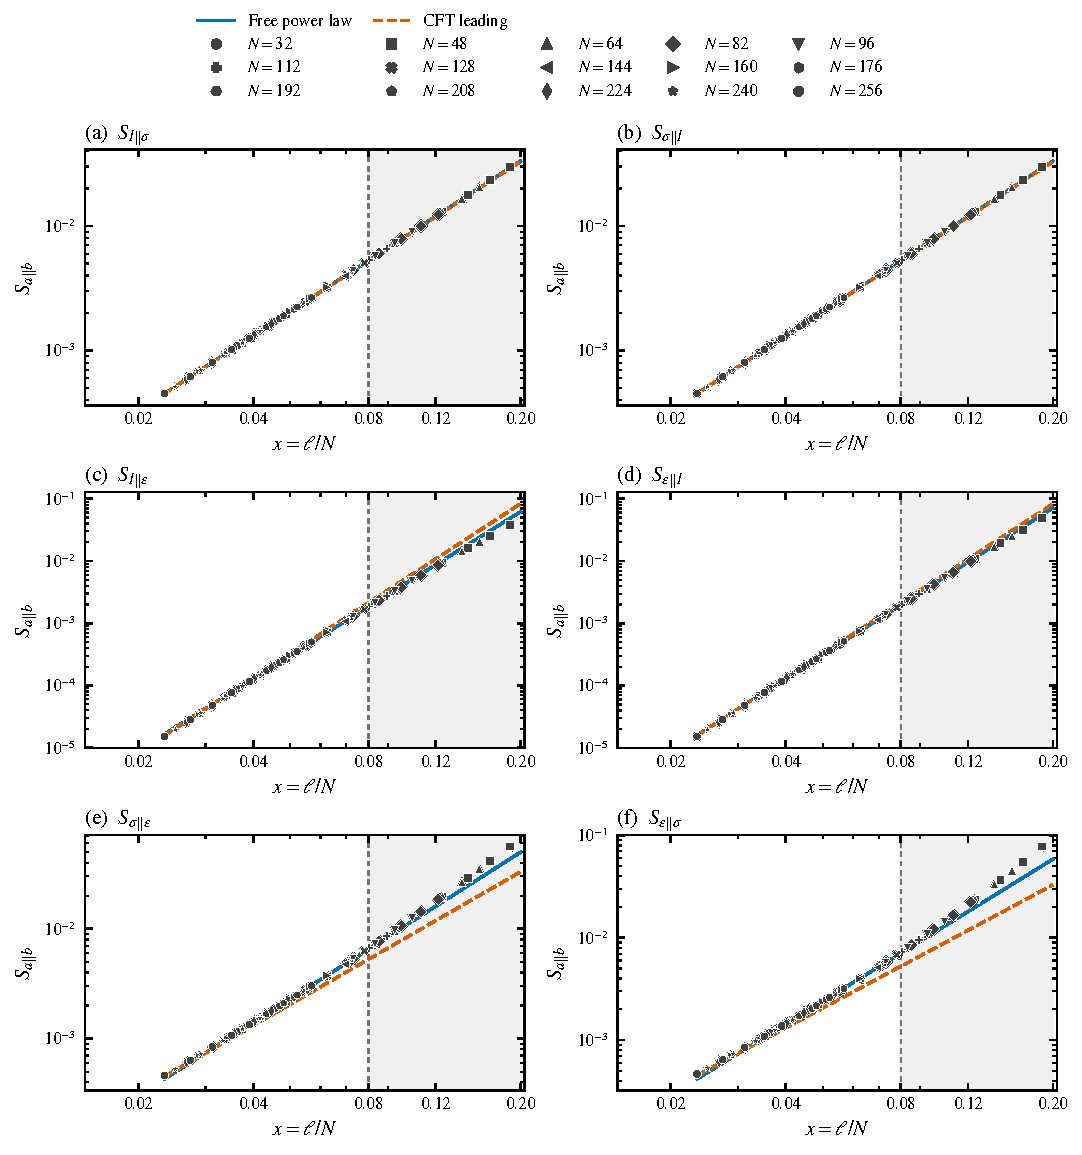
\includegraphics[width=.95\linewidth]{../figs/ising_primary_fits.pdf}
\caption{Historical Ising primary relative entropy $S_{a\Vert b}$ for
all six directions. Markers identify the 15 system sizes through
$N=256$ in Eq.~\eqref{eq:large-grid}; $\ell=6,\ldots,10$.
Each panel shows 70 observations with $x=\ell/N\leq0.20$.
Only the 51 observations at $x\leq0.08$ enter the unweighted
least-squares fits in Eq.~\eqref{eq:primary-fit-ansatz}.
The vertical line and shading mark the cutoff and the extrapolation
region containing 19 observations. Blue solid lines show the free
power law $F=\widehat Cx^{\widehat\alpha}$; both parameters
are optimized independently for each direction. Orange dashed
lines show the analytical CFT leading-order prediction, with no fitted parameters. For panels (c,d),
$\alpha_{\rm CFT}=4$ and $B_{ab}=8\pi^4/15$; elsewhere
$\alpha_{\rm CFT}=2$ and $B_{ab}=\pi^2/12$.
Table~\ref{tab:ising-primary-all-fits} compares both fitted
parameters with these analytical values.
The data use exact Jordan--Wigner primaries of the critical
periodic-spin Hamiltonian $H=-\sum XX-\sum Z$,
natural logarithms, and target-logarithm floor $10^{-15}$.
Both axes are logarithmic. The fitted exponent is a free real
number and the coefficient is positive; no additional powers enter.}
\label{fig:ising-primary-fits}
\end{figure}

\begin{figure}[p]\centering
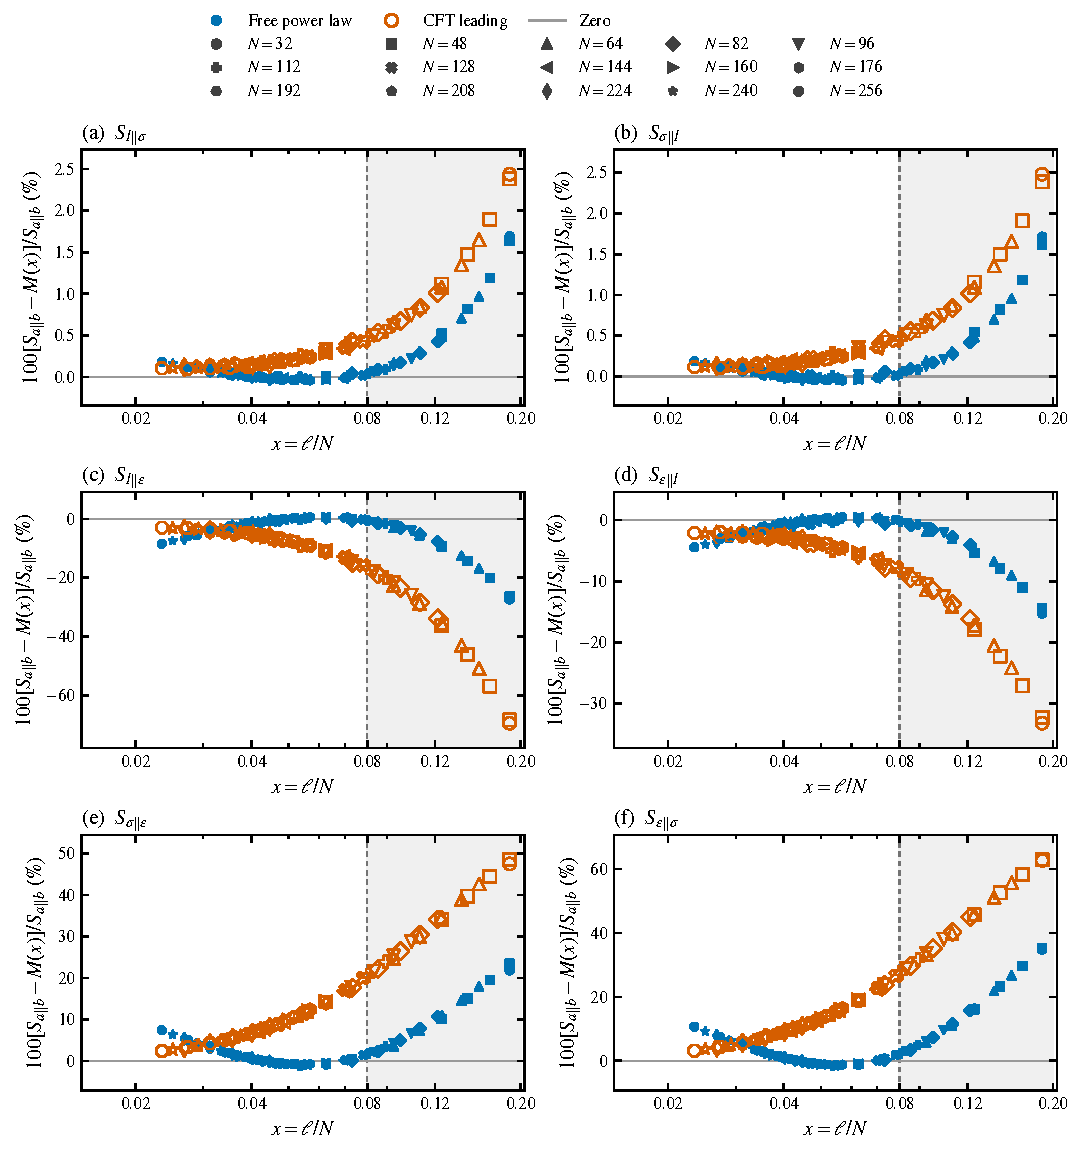
\includegraphics[width=.95\linewidth]{../figs/ising_primary_residuals.pdf}
\caption{Signed percentage residuals for the Ising primary
comparisons in Fig.~\ref{fig:ising-primary-fits}. Blue filled markers
denote the free power law and orange open markers the analytical
leading prediction. Marker shapes identify the 15 sizes in
Eq.~\eqref{eq:large-grid}, with
$\ell=6,\ldots,10$. The ordinate is
$\eta_i=100[S_{a\Vert b}(x_i)-M(x_i)]/S_{a\Vert b}(x_i)$,
where $M=F$ or $F_{\rm CFT}$,
from Eq.~\eqref{eq:primary-fit-residual}; zero means exact agreement.
The ordinate is linear throughout, with ticks showing signed percentage
values directly; $x$ is logarithmic.
All 70 displayed observations per direction satisfy $x\leq0.20$.
Only 51 at $x\leq0.08$ determine the fits and table metrics;
the 19 shaded-region observations test extrapolation.
The free fit has two jointly optimized parameters,
$F=\widehat Cx^{\widehat\alpha}$.
Only the analytical comparison uses $\alpha_{\rm CFT}=4$,
$B_{ab}=8\pi^4/15$ in (c,d), and $\alpha_{\rm CFT}=2$, $B_{ab}=\pi^2/12$
otherwise. The exact PBC Ising states, natural
logarithms and target floor $10^{-15}$ are as in
Fig.~\ref{fig:ising-primary-fits}; coefficients, exponents, RMSE and
CV RMSE appear in Table~\ref{tab:ising-primary-all-fits}.}
\label{fig:ising-primary-residuals}
\end{figure}

\begin{figure}[p]\centering
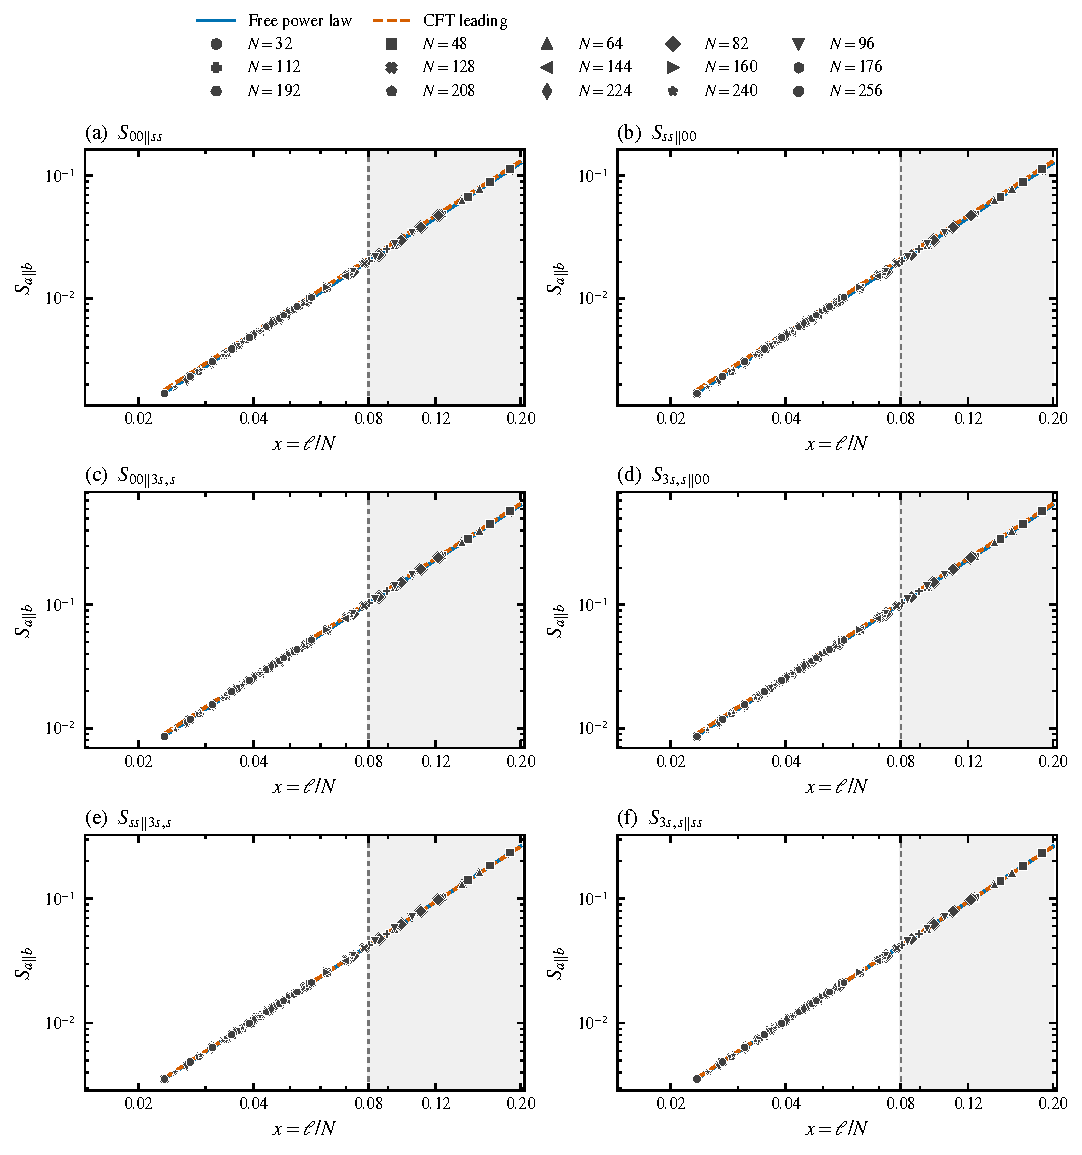
\includegraphics[width=.95\linewidth]{../figs/boson_primary_fits.pdf}
\caption{Historical compact-boson primary relative entropy for all six
directions among charges $(0,0)$, $(s,s)$ and $(3s,s)$,
$s=1/\sqrt2$. Markers identify the 15 sizes through $N=256$
in Eq.~\eqref{eq:large-grid}; $\ell=6,\ldots,10$.
Each panel displays 70 observations at $x\leq0.20$.
The 51 observations at $x\leq0.08$ determine the unweighted
least-squares fits; the vertical line and shading mark the 19
observations outside the fit window. Blue solid lines show
$F=\widehat Cx^{\widehat\alpha}$ from
Eq.~\eqref{eq:primary-fit-ansatz}, with both coefficient and exponent
optimized. Orange dashed lines show the analytical CFT leading-order
predictions, with no fitted parameters: $\alpha_{\rm CFT}=2$ and
$B_{ab}=\pi^2/3$ in (a,b), $5\pi^2/3$ in (c,d), and $2\pi^2/3$ in (e,f).
Table~\ref{tab:boson-primary-all-fits} compares both fitted
parameters with the analytical values.
The normalized vertex/Jastrow states use the unit circle,
$q=2$, $w_1=0$, $W=10^8$, and 100-decimal-digit Pfaffian
construction, without orthogonalization, as in
Sec.~\ref{sec:primary-numerics}.
All logarithms are natural and the target-logarithm floor
is $10^{-15}$. Both axes are logarithmic. The fit has a positive
coefficient and a free real exponent, with no additional terms.}
\label{fig:boson-primary-fits}
\end{figure}

\begin{figure}[p]\centering
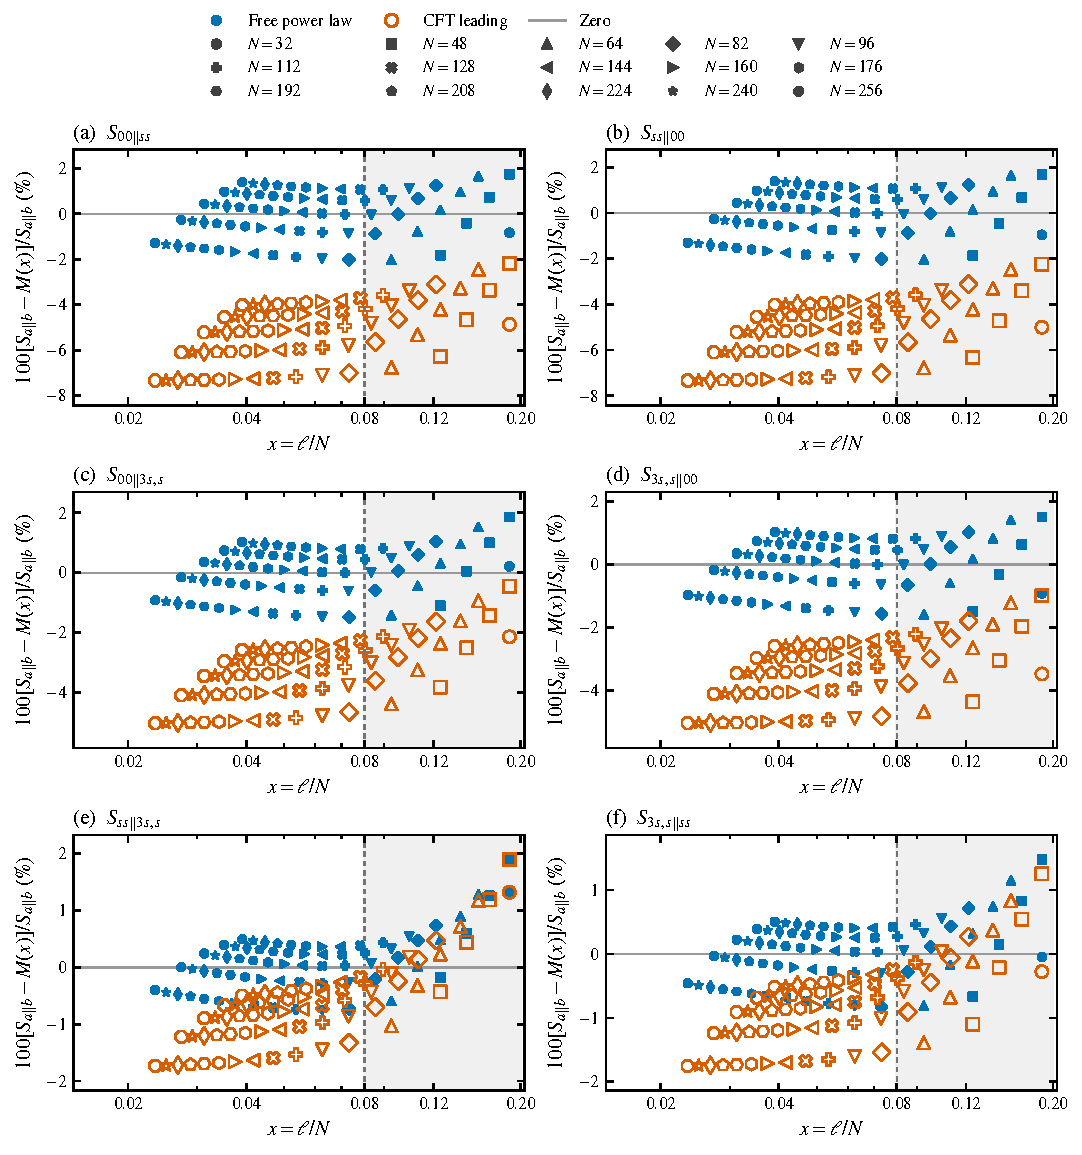
\includegraphics[width=.95\linewidth]{../figs/boson_primary_residuals.pdf}
\caption{Signed percentage residuals for the compact-boson
primary comparisons in Fig.~\ref{fig:boson-primary-fits}.
Blue filled markers denote the free power law; orange open markers
denote the analytical leading term.
The ordinate is $100[S_{a\Vert b}-M]/S_{a\Vert b}$,
where $M=F$ or $F_{\rm CFT}$,
as in Eq.~\eqref{eq:primary-fit-residual}. The vertical scale is linear
throughout, with ticks showing signed percentage values directly;
$x$ is logarithmic. Markers identify the 15 sizes in
Eq.~\eqref{eq:large-grid}, with $\ell=6,\ldots,10$.
All 70 observations per direction at $x\leq0.20$ are shown;
51 at $x\leq0.08$ enter the fits and metrics, while 19 lie
in the shaded extrapolation region. The two-parameter fit is
$F=\widehat Cx^{\widehat\alpha}$; its exponent is not
fixed. The analytical comparison uses $\alpha_{\rm CFT}=2$
and $B_{ab}=\pi^2/3$, $5\pi^2/3$, $2\pi^2/3$ in the top, middle and bottom rows.
The vertex charges, $q=2$,
unit-circle sites, $w_1=0$, $W=10^8$, 100-digit construction,
absence of orthogonalization, natural logarithms and
target floor $10^{-15}$ are as in Fig.~\ref{fig:boson-primary-fits}.
Table~\ref{tab:boson-primary-all-fits} compares fitted coefficients
and exponents with theory and gives RMSE and size-based CV RMSE.}
\label{fig:boson-primary-residuals}
\end{figure}
\clearpage
